
    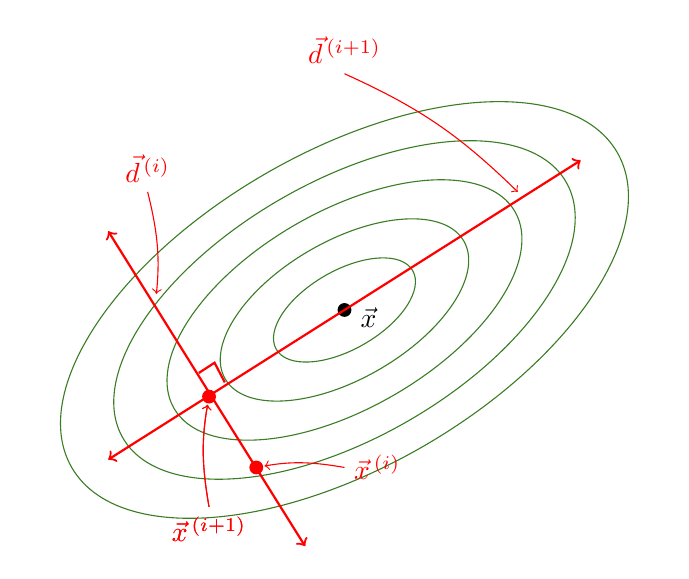
\begin{tikzpicture}
        \foreach \size in {1, 1.75, ..., 4} {
            \draw[OliveGreen, scale=\size, rotate=30] (0,0) ellipse (1cm and .5cm);
        };
        % \node[circle, inner sep=0, minimum size=5pt,fill, label={30:$\vec{x}$}]() at (0,0){};
        \node[circle, inner sep=0, minimum size=5pt,fill, label={[yshift=2mm]-30:$\vec{x}$}]() at (0,0){};

        \draw[<->, thick, red] (3, 1.9) -- (-3, -1.9);
        \draw[<->, thick, red] (-3, 1) -- (-.5, -3);

        \node[red, circle, inner sep=0, minimum size=5pt,fill] () at (-1.12, -2){};
        \node[red, circle, inner sep=0, minimum size=5pt,fill] () at (-1.72, -1.1){};
        \draw[thick, red] (-1.85, -0.8) -- (-1.65, -0.67) -- (-1.52, -0.92);

        \draw[<-, shorten <=3pt, red] (-1.12, -2) to[bend left=10] (0, -2) node[right] () {$\vec{x}^{\,(i)}$};
        \draw[<-, shorten <=3pt, red] (-1.72, -1.1) to[bend right=10] (-1.72, -2.5) node[below] () {$\vec{x}^{\,(i+1)}$};
        \draw[<-, shorten <=3pt, red] (-1.72, -1.1) to[bend right=10] (-1.72, -2.5) node[below] () {$\vec{x}^{\,(i+1)}$};
        \draw[<-, shorten <=3pt, red] (-2.4, .1) to[bend right=10] (-2.5, 1.5) node[above] () {$\vec{d}^{\,(i)}$};
        \draw[<-, red] (2.2, 1.5) to[bend right=10] (0, 3) node[above] () {$\vec{d}^{\,(i+1)}$};

    \end{tikzpicture}
